\documentclass[11pt,a4paper]{article}
\usepackage[margin=2.2cm]{geometry}
\usepackage{booktabs}
\usepackage{microtype}
\usepackage{parskip}
\usepackage{hyperref}
\usepackage{xcolor}
\usepackage{amsmath,amssymb}
\usepackage{caption}
\usepackage{tikz}
\usetikzlibrary{arrows.meta, positioning, fit, shapes.geometric}
\usepackage[numbers,sort&compress]{natbib}

\title{\textbf{Audio-Visual Information Bottleneck with Qwen3-Omni}\\
       \large Experiment Report}
\author{Souleiman Sbais}
\date{June 2026}

\begin{document}
\maketitle
\tableofcontents
\vspace{1em}\hrule\vspace{1em}

% ─────────────────────────────────────────────────────────────────────────────
\section{Motivation}

Large audio-visual language models generate confident responses even when a
required modality is absent or corrupted.  This \emph{hallucination under
modal degradation} is well-documented: models trained to always answer learn
to ignore missing evidence and rely on language priors instead
\cite{mad2026,dpa2026}.  We address this with a \textbf{fail-safe mechanism}:
the model should abstain when its bottlenecked representation carries too
little task-relevant information, rather than guess.

The approach builds on two ideas:
(i) the \textbf{Variational Information Bottleneck} (VIB) \cite{alemi2017vib},
which learns a compressed stochastic representation $Z$ of an input modality
by trading off task accuracy against channel capacity; and
(ii) \textbf{Direct Preference Optimization} (DPO) \cite{rafailov2023dpo},
which steers the model's output distribution toward abstention on corrupted
inputs without explicit reward modelling.

% ─────────────────────────────────────────────────────────────────────────────
\section{Architecture}

\subsection{Backbone: Qwen3-Omni-30B}

The base model is \textbf{Qwen3-Omni-30B-A3B} \cite{qwen3omni2025}, a
30B-parameter Mixture-of-Experts multimodal LLM with a native audio-visual
encoder.  The model accepts interleaved video and audio tokens alongside text
and autoregressively generates text responses.  We keep the entire backbone
\emph{frozen} throughout all experiments; only the lightweight components
described below are trained.

\subsection{Video Information Bottleneck}

A trainable \textbf{bottleneck head} is inserted between the frozen video
encoder's output and the LLM's token sequence.  It parametrises a diagonal
Gaussian over the video representation:
\[
  q(z \mid v) = \mathcal{N}\!\left(\mu_\phi(v),\;\operatorname{diag}(\sigma^2_\phi(v))\right)
\]
During training, $z \sim q(z|v)$ via the reparametrisation trick.  At
inference (noise off), $z = \mu_\phi(v)$.  The bottleneck objective is:
\[
  \mathcal{L} = \underbrace{\mathcal{L}_\text{NLL}(y \mid z, a, x)}_{\text{task accuracy}}
              \;+\;\beta \cdot \underbrace{D_\text{KL}\!\left(q(z|v)\;\|\;\mathcal{N}(0,I)\right)}_{\text{video compression}}
\]
where $a$ is the audio stream and $x$ is the text prompt.  The KL term
penalises information flowing through the video channel: under clean video
$\beta$-KL is the rate cost; under corrupted video the posterior collapses
toward the prior, making $z$ uninformative.

\begin{figure}[h]
\centering
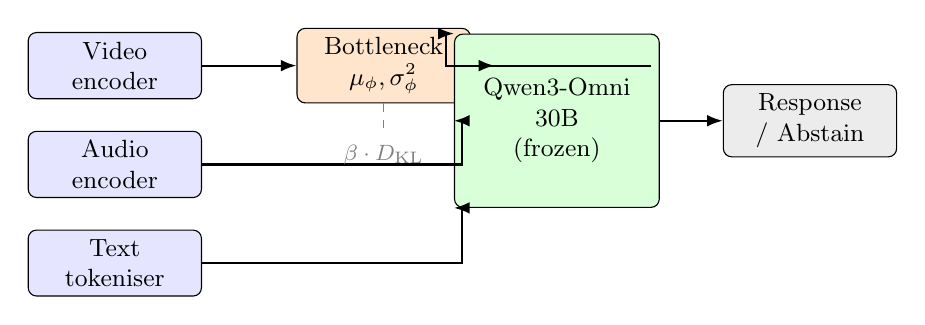
\begin{tikzpicture}[
  box/.style={draw, rounded corners=3pt, minimum width=2.2cm,
              minimum height=0.75cm, align=center, font=\small},
  arrow/.style={-{Latex[length=2mm]}, thick},
  node distance=0.5cm and 1.0cm
]
  % inputs
  \node[box, fill=blue!10]  (vid) {Video\\encoder};
  \node[box, fill=blue!10, below=0.4cm of vid] (aud) {Audio\\encoder};
  \node[box, fill=blue!10, below=0.4cm of aud] (txt) {Text\\tokeniser};

  % bottleneck
  \node[box, fill=orange!20, right=1.2cm of vid] (bn)
        {Bottleneck\\$\mu_\phi,\sigma^2_\phi$};
  \node[right=0.3cm of bn, font=\small] (sample) {$z\!\sim\!\mathcal{N}(\mu,\sigma^2)$};

  % LLM
  \node[box, fill=green!15, right=3.2cm of vid, yshift=-0.7cm, minimum width=2.6cm,
        minimum height=2.2cm] (llm) {Qwen3-Omni\\30B\\(frozen)};

  % output
  \node[box, fill=gray!15, right=0.8cm of llm] (out) {Response\\/ Abstain};

  % arrows
  \draw[arrow] (vid) -- (bn);
  \draw[arrow] (bn) -- (sample);
  \draw[arrow] (sample.east) -| ([xshift=-0.1cm]llm.north west) -- (llm.north west);
  \draw[arrow] (aud.east) -- ++(0.3,0) -| ([xshift=0.1cm]llm.west) -- (llm.west);
  \draw[arrow] (txt.east) -- ++(0.3,0) -| ([xshift=0.1cm]llm.south west) -- (llm.south west);
  \draw[arrow] (llm) -- (out);

  % KL annotation
  \draw[dashed, gray] (bn.south) -- ++(0,-0.4)
    node[below, font=\footnotesize, gray] {$\beta\cdot D_\text{KL}$};
\end{tikzpicture}
\caption{Architecture overview.  Only the bottleneck head ($\mu_\phi, \sigma^2_\phi$)
and optional LoRA adapters are trainable; everything else is frozen.}
\end{figure}

\subsection{Abstention Training (DPO)}

After the bottleneck pre-training, a DPO stage teaches the model \emph{when}
to abstain.  Preference pairs are constructed by corrupting the video channel
in three ways seen during training: zeroing all frames (\texttt{vid\_zero}),
replacing with the channel mean (\texttt{vid\_mean}), and the clean original
(\texttt{identity}).  For each pair the chosen response is abstention
(``I can't tell'') on a corrupted input, and the rejected response is the
model's own overconfident answer.  The DPO loss \cite{rafailov2023dpo} is:
\[
  \mathcal{L}_\text{DPO} = -\mathbb{E}\!\left[
    \log\sigma\!\left(\beta\log\frac{\pi_\theta(y_w|x)}{\pi_\text{ref}(y_w|x)}
    - \beta\log\frac{\pi_\theta(y_l|x)}{\pi_\text{ref}(y_l|x)}\right)
  \right]
\]
At evaluation, abstention is detected by teacher-forcing the NLL of three
continuations --- the real answer options plus ``I can't tell'' --- and
picking the minimum-NLL response.

\subsection{Conditions}

\begin{center}
\begin{tabular}{lll}
\toprule
\textbf{Condition} & \textbf{Modalities bottlenecked} & \textbf{Training} \\
\midrule
Untrained baseline     & none & --- \\
LoRA baseline          & none & NLL (LoRA) \\
Video bottleneck base  & video only & NLL + $\beta$KL \\
Video bottleneck DPO   & video only & VIB then DPO \\
Video bottleneck SFT   & video only & VIB then SFT abstention \\
AV bottleneck DPO      & video + audio & VIB then DPO \\
\bottomrule
\end{tabular}
\end{center}

% ─────────────────────────────────────────────────────────────────────────────
\section{Benchmarks}

\textbf{AVQA} \cite{yang2022avqa}: 57,015 video clips from VGGSound \cite{vggsound2020},
4-way multiple-choice (letters A--D), questions categorised as
View / Sound / Both.  Because VGGSound is curated around sound events, these
questions are predominantly answerable from audio alone.

\textbf{AVHBench} \cite{avhbench2024}: open-domain clips from VGGSound and
AudioCaps, binary yes/no, three task types --- AV Matching,
Audio-driven Video Hallucination, Video-driven Audio Hallucination.
Both modalities are genuinely required, making it the more faithful substrate
for the fail-safe abstention experiment.

% ─────────────────────────────────────────────────────────────────────────────
\section{Results on AVQA}

\subsection{Accuracy}

\begin{center}
\begin{tabular}{lrrrr}
\toprule
\textbf{Model} & \textbf{Acc (\%)} & \textbf{Mean NLL} & \textbf{Mean KL (video)} & $n$ \\
\midrule
Untrained baseline & \textbf{94.0} & 0.112 & 2904.9 & 300 \\
Video bottleneck   & 93.3          & 0.105 & \textbf{1601.4} & 300 \\
LoRA baseline      & 91.7          & 0.125 & 2904.9 & 300 \\
\bottomrule
\end{tabular}
\end{center}

The bottleneck halved the video KL (2905 $\to$ 1601) at negligible accuracy
cost ($-0.7$ pp on $n{=}300$).  LoRA fine-tuning slightly degraded accuracy,
consistent with the base model being near ceiling on this audio-dominated
sample.

\subsection{Abstention (Risk-Coverage)}

\begin{center}
\small
\begin{tabular}{llrrl}
\toprule
\textbf{Model} & \textbf{Corruption} & \textbf{Coverage} & \textbf{Risk} & \textbf{Group} \\
\midrule
Video bottleneck DPO & identity   & 100.0\% &  8.7\% & train \\
                     & vid\_zero  &  99.3\% &  8.1\% & train \\
                     & vid\_mean  &  98.0\% & 11.6\% & train \\
                     & vid\_noise & 100.0\% &  8.7\% & held-out \\
                     & vid\_scale & 100.0\% &  6.0\% & held-out \\
\midrule
AV bottleneck DPO    & identity   & 100.0\% & 11.3\% & train \\
                     & vid\_zero  &  93.3\% &  8.6\% & train \\
                     & vid\_mean  &  86.7\% & 16.9\% & train \\
                     & vid\_noise &  99.3\% & 10.1\% & held-out \\
                     & vid\_scale & 100.0\% &  8.0\% & held-out \\
\midrule
Video bottleneck SFT & identity   & 100.0\% &  8.7\% & train \\
                     & vid\_mean  &  88.0\% &  9.8\% & train \\
\bottomrule
\end{tabular}
\end{center}

Abstention did not emerge on AVQA: coverage stays near 100\% and risk stays
$\approx 8$--$17$\% regardless of video corruption severity.  The cause is an
ecological mismatch --- VGGSound questions are largely answerable from audio
alone, so corrupting the video does not increase the model's error rate, and
there is therefore no information-theoretic incentive to abstain.  The negative
control confirms this: corrupting audio also leaves coverage and risk
essentially unchanged.

% ─────────────────────────────────────────────────────────────────────────────
\section{Ongoing: AVHBench Evaluation}

The same five checkpoints are now being evaluated on AVHBench \cite{avhbench2024}
with the parallel 6-GPU eval script.  Because both modalities are genuinely
required for AVHBench's judgment tasks, we expect: (i) risk to rise under
\texttt{vid\_zero}/\texttt{vid\_mean}; (ii) the DPO models to begin abstaining
(coverage drops) while the baselines maintain coverage with elevated risk;
and (iii) audio corruption (\texttt{aud\_zero}/\texttt{aud\_mean}) to also
affect coverage for audio-driven tasks, unlike the AVQA case.

% ─────────────────────────────────────────────────────────────────────────────
\bibliographystyle{unsrtnat}
\bibliography{refs}

\end{document}
